% 課題別の逆引きガイドの流れ図（en 版）。reader_guide_flow.tex から scripts/gen-reader-guide-flow-tex.py で生成。
% reader_guide_flow.pdf（PDF用）と reader_guide_flow.png（Web・EPUB用）の元データです。
% 生成: scripts/build-reader-guide-flow.sh
\documentclass[uplatex,dvipdfmx,class=ujarticle,border=1mm]{standalone}
\usepackage[deluxe,uplatex]{otf}
\usepackage[T1]{fontenc}
\usepackage[noalphabet,unicode]{pxchfon}
\setgothicfont{BIZUDGothic-Regular.ttf}
\setboldgothicfont{BIZUDGothic-Bold.ttf}
\renewcommand{\sfdefault}{phv}
\renewcommand\familydefault{\sfdefault}
\renewcommand\kanjifamilydefault{\gtdefault}
\usepackage{tikz}
\usetikzlibrary{positioning,arrows.meta}
\definecolor{ink}{HTML}{2B2B2B}
\definecolor{panel}{HTML}{F2F4F7}
\definecolor{sub}{HTML}{55606E}

\newcommand{\colw}{33mm}
\newcommand{\colgap}{36mm}

\begin{document}
\hyphenpenalty=10000 \exhyphenpenalty=10000 \tolerance=9999 \emergencystretch=3em
\kanjiskip=.05zw plus.5pt minus.5pt\xkanjiskip=0pt
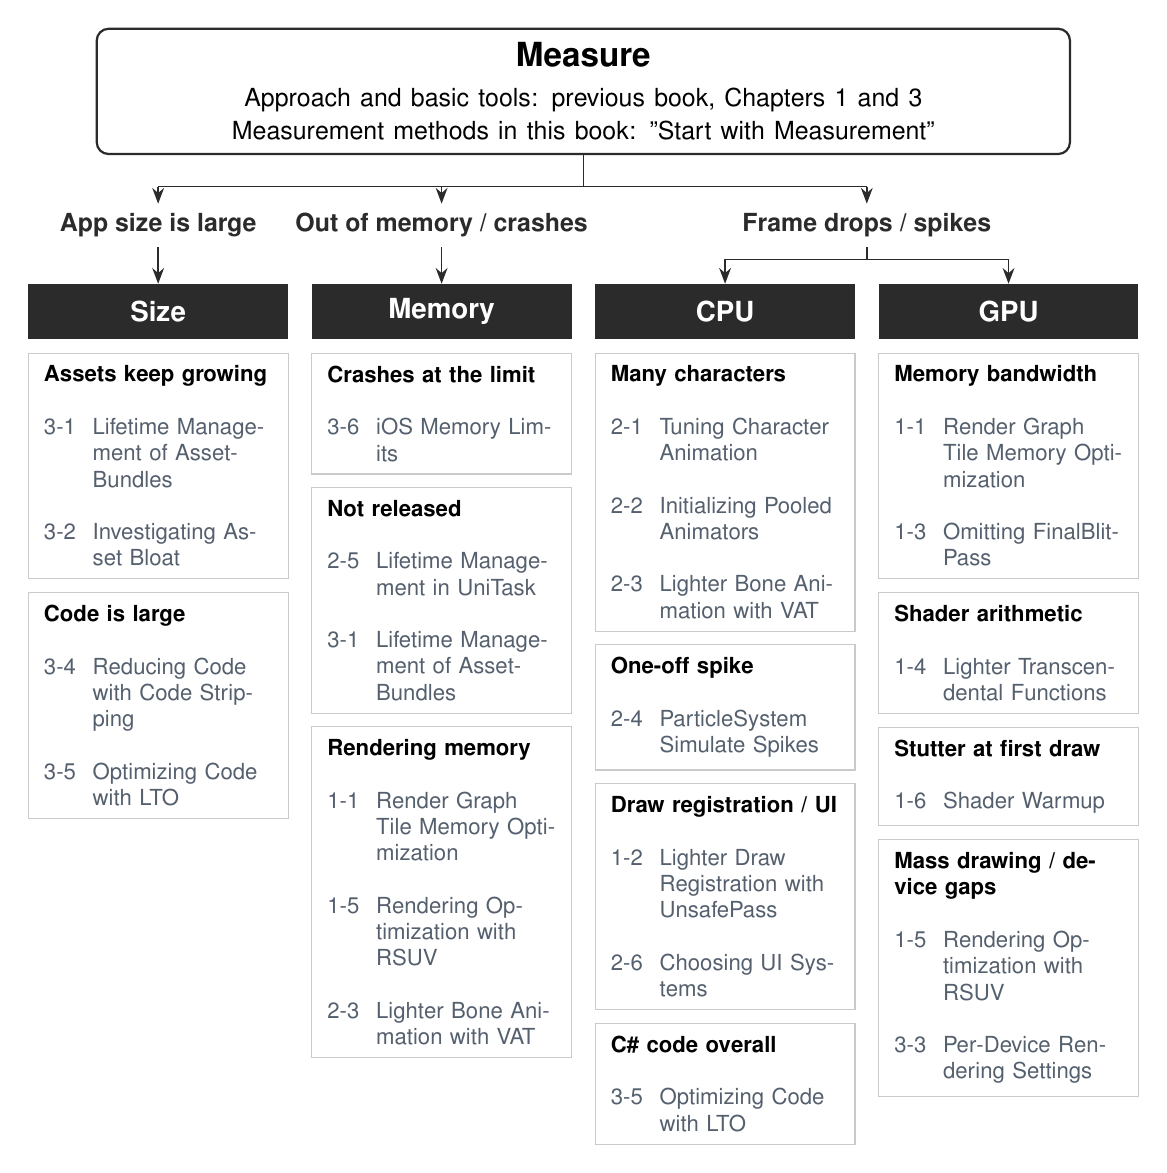
\begin{tikzpicture}[
  font=\sffamily\gtfamily,
  line/.style={draw=ink, line width=0.6pt},
  arrow/.style={line, -{Stealth[length=2mm]}},
  measure/.style={draw=ink, line width=0.8pt, rounded corners=1.5mm, fill=white,
    align=center, inner sep=1.8mm, text width=120mm},
  symptom/.style={align=center, font=\small\bfseries\gtfamily, text=ink},
  section/.style={fill=ink, text=white, font=\bfseries\gtfamily, minimum height=7mm,
    text width=\colw, align=center, inner sep=0pt},
  leaf/.style={fill=white, draw=ink!25, line width=0.4pt, text width=\colw-4mm,
    align=left, inner xsep=2mm, inner ysep=1.6mm, font=\footnotesize\gtfamily},
]
% 計測
\node[measure] (measure) at (1.5*\colgap, 0) {%
  {\large\bfseries Measure}\\[0.8mm]
  {\small Approach and basic tools: previous book, Chapters 1 and 3\qquad
  Measurement methods in this book: "Start with Measurement"}};

% 症状
\node[symptom] (s1) at (0, -17mm) {App size is large};
\node[symptom] (s2) at (\colgap, -17mm) {Out of memory / crashes};
\node[symptom] (s3) at (2.5*\colgap, -17mm) {Frame drops / spikes};

\draw[line] (measure.south) -- ++(0, -4mm) coordinate (bus);
\draw[line] (0, 0 |- bus) -- (2.5*\colgap, 0 |- bus);
\foreach \s in {s1, s2, s3} \draw[arrow] (\s |- bus) -- (\s.north);

% 課題（本書の節）
\foreach \x/\name/\label in {0/c1/Size, 1/c2/Memory, 2/c3/CPU, 3/c4/GPU}
  \node[section] (\name) at (\x*\colgap, -28mm) {\label};
\draw[arrow] (s1.south) -- (c1.north);
\draw[arrow] (s2.south) -- (c2.north);
\draw[line] (s3.south) -- ++(0, -1.6mm) coordinate (split);
\draw[line] (c3 |- split) -- (c4 |- split);
\draw[arrow] (c3 |- split) -- (c3.north);
\draw[arrow] (c4 |- split) -- (c4.north);

% 症状ごとの章
% \leafitem{上のノード}{名前}{症状}{章}
% \ch{部-章}{短縮した章タイトル}：症状と章、章と章の間を1行空け、2行目以降は番号の後ろにそろえる
\newcommand{\ch}[2]{\par
  \vspace{\baselineskip}
  \hangindent=2.2em\hangafter=1
  \noindent\makebox[2.2em][l]{#1}#2}
\newcommand{\leafitem}[4]{%
  \node[leaf, below=1.6mm of #1] (#2) {{\bfseries #3}\par{\color{sub}#4\par}};}

\leafitem{c1}{c1a}{Assets keep growing}{\ch{3-1}{Lifetime Management of AssetBundles}\ch{3-2}{Investigating Asset Bloat}}
\leafitem{c1a}{c1b}{Code is large}{\ch{3-4}{Reducing Code with Code Stripping}\ch{3-5}{Optimizing Code with LTO}}

\leafitem{c2}{c2a}{Crashes at the limit}{\ch{3-6}{iOS Memory Limits}}
\leafitem{c2a}{c2b}{Not released}{\ch{2-5}{Lifetime Management in UniTask}\ch{3-1}{Lifetime Management of AssetBundles}}
\leafitem{c2b}{c2c}{Rendering memory}{\ch{1-1}{Render Graph Tile Memory Optimization}\ch{1-5}{Rendering Optimization with RSUV}\ch{2-3}{Lighter Bone Animation with VAT}}

\leafitem{c3}{c3a}{Many characters}{\ch{2-1}{Tuning Character Animation}\ch{2-2}{Initializing Pooled Animators}\ch{2-3}{Lighter Bone Animation with VAT}}
\leafitem{c3a}{c3b}{One-off spike}{\ch{2-4}{ParticleSystem Simulate Spikes}}
\leafitem{c3b}{c3c}{Draw registration / UI}{\ch{1-2}{Lighter Draw Registration with UnsafePass}\ch{2-6}{Choosing UI Systems}}
\leafitem{c3c}{c3d}{C\# code overall}{\ch{3-5}{Optimizing Code with LTO}}

\leafitem{c4}{c4a}{Memory bandwidth}{\ch{1-1}{Render Graph Tile Memory Optimization}\ch{1-3}{Omitting FinalBlitPass}}
\leafitem{c4a}{c4b}{Shader arithmetic}{\ch{1-4}{Lighter Transcendental Functions}}
\leafitem{c4b}{c4c}{Stutter at first draw}{\ch{1-6}{Shader Warmup}}
\leafitem{c4c}{c4d}{Mass drawing / device gaps}{\ch{1-5}{Rendering Optimization with RSUV}\ch{3-3}{Per-Device Rendering Settings}}
\end{tikzpicture}
\end{document}
